\begin{ExerciseList}

  \setcounter{Exercise}{0}

  \section{Lab 5: File system, Spawn and Shell}

  \subsection{实验目的}

  在本实验中,我们将实现spawn一个加载和运行磁盘可执行文件的库调用。然后充实我们的内核和库操作系统,在控制台上运行一个shell。这些功能需要一个文件系统,本实验将介绍一个简单的读/写文件系统。

  \subsection{实验过程}

  \subsubsection{第一部分:文件系统实现}


  实验指导书首先简单介绍了一般文件系统的结构,包括扇区、块、超级块、块位图、文件元数据和目录的概念。在jos中不会实现一个真实的文件系统的全部功能。我们实现的操作系统不会包含权限的限制,默认是单用户操作系统。组织文件时不使用inode,而是直接使用元数据。为了存储更大的文件将使用一层间接块。

  \textbf{磁盘访问}

  当前jos操作系统中的文件系统环境需要能够访问磁盘,但我们还没有在内核中实现任何磁盘访问功能。除了采用传统的“单块”操作系统策略,即将IDE磁盘驱动程序与必要的系统调用一起添加到内核中以允许文件系统访问它之外,我们还将IDE磁盘驱动程序作为用户级文件的一部分系统环境。我们仍然需要稍微修改内核,以便进行设置,以便文件系统环境具有实现本身磁盘访问所需的权限。”


  \Exercise{首先要打开文件系统访问I/O的权限,在创建进程时判断如果是文件系统的进程,那么给与I/O访问权限。}

  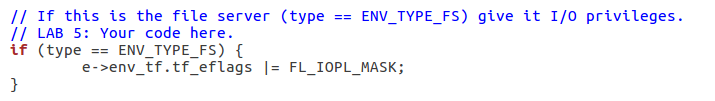
\includegraphics[width=6in]{figures/lab5/image64.png}

  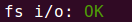
\includegraphics[width=6in]{figures/lab5/image65.png}

  问题1:

  回答:不用,切换进程时调用的pop\_tf函数中的iret指令恢复了包括eflags的寄存器。

  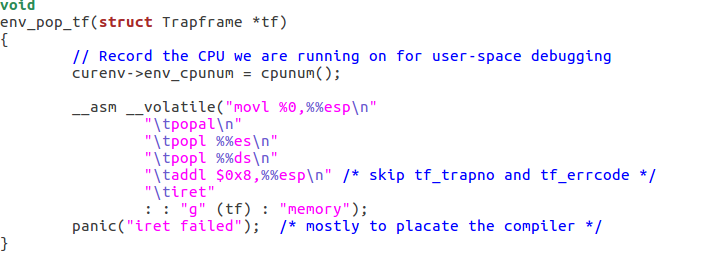
\includegraphics[width=6in]{figures/lab5/image67.png}

  \textbf{块缓存}

  Jos中我们通过缓存技术来实现访问磁盘块。该机制可以支持最大3GB的磁盘。

  我们将文件系统服务进程的虚拟地址空间(0x10000000 (DISKMAP)到0xD0000000 (DISKMAP+DISKMAX))对应到磁盘的地址空间(3GB)。

  由于现代磁盘大于3GB,在32位机器上的真正的文件系统实现会很麻烦。这种缓冲区高速缓存管理方法在64位地址空间的机器上仍然是合理的。

  映射方法:我们假装整个磁盘都已经被缓存到内存中,当我们想访问虚拟空间中的一个页时,由于虚拟空间还没有被映射,会发生页错误。在页错误处理程序中则会实际进行磁盘块到虚拟地址的映射并将该块磁盘内容缓存到内存中。

  此时就可以恢复文件系统进程进行正常的文件访问。

  \Exercise{Exercise2}

  Bc\_pgfault函数负责处理页面错误,处理的同时进行页面映射并从磁盘中缓存对应的块到内存中。

  处理的步骤:

  \begin{enumerate}
  \item 根据地址计算出对应的blockno(块编号)
  \item 检查地址范围是否超出(0x10000000 (DISKMAP)到0xD0000000 (DISKMAP+DISKMAX))的映射边界
  \item 检查块编号是否超出块数
  \item 将地址对齐到页起始位置
  \item 页面映射
  \item 调用ide\_read函数读取缓存块对应的数个磁盘页到内存中
  \item 更新脏位
  \end{enumerate}

  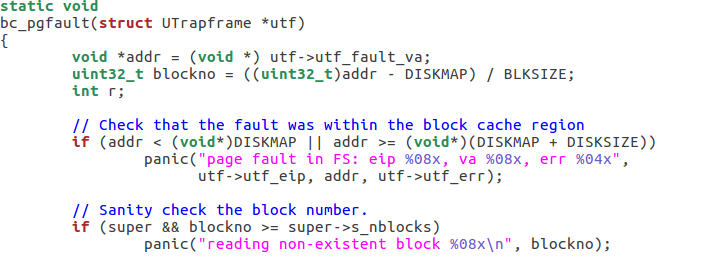
\includegraphics[width=6in]{figures/lab5/image69.png}

  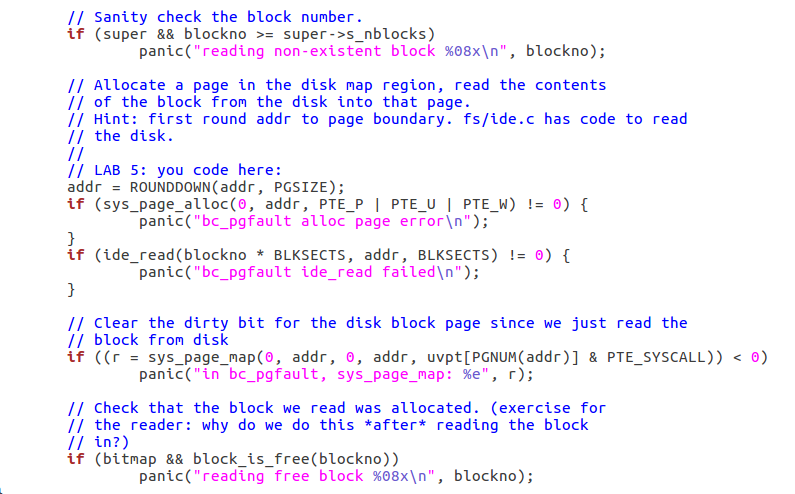
\includegraphics[width=6in]{figures/lab5/image70.png}

  Flush\_block函数负责将缓存中的块写回到磁盘中。

  处理步骤:

  \begin{enumerate}
  \item 根据地址计算出对应的blockno(块编号)
  \item 检查地址范围是否超出(0x10000000 (DISKMAP)到0xD0000000 (DISKMAP+DISKMAX))的映射边界
  \item 检查如果对应块没有映射就不写回
  \item 检查如果对应块不是脏块(没有发生改动)就不写回
  \item 最后将缓存写回到磁盘,检查是否成功并更新脏位
  \end{enumerate}

  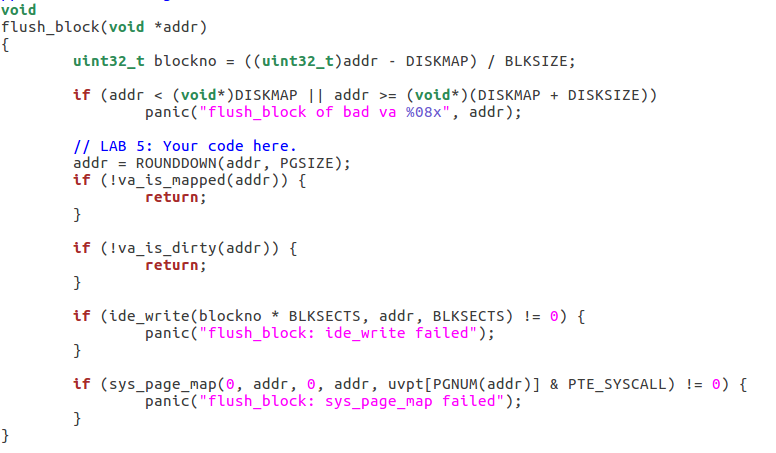
\includegraphics[width=6in]{figures/lab5/image71.png}

  通过make grade检查是否成功

  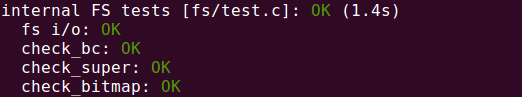
\includegraphics[width=6in]{figures/lab5/image72.png}

  \textbf{块分配表}

  Block bitmap记录磁盘上的一块是否写有内容。在fs\_init设置bitmap指针之后,我们可以将其bitmap视为一个打包的位数组,每个磁盘块对应一个位。我们可以使用block\_is\_free函数检查给定块在位图中是否被标记空的。

  \Exercise{Exercise3}

  依次遍历所有bitmap位,当发现bitmap的第i位为1(表示能用)时将此位赋0并返回块号i。

  \textbf{文件操作}

  在fs / fs.c中提供了各种函数来实现管理File的基本结构,扫描和管理目录文件的条目,从根目录文件系统来解析绝对路径名。

  \Exercise{此步需要实现实现 file\_block\_walk 和file\_get\_block函数。}

  Fs.c文件中编写了与文件操作有关的一系列操作,例如浏览目录,解析路径等。

  file\_block\_walk函数寻找一个文件结构f中的第fileno个块指向的磁盘块编号放入ppdiskbno。类似于遍历目录结构。

  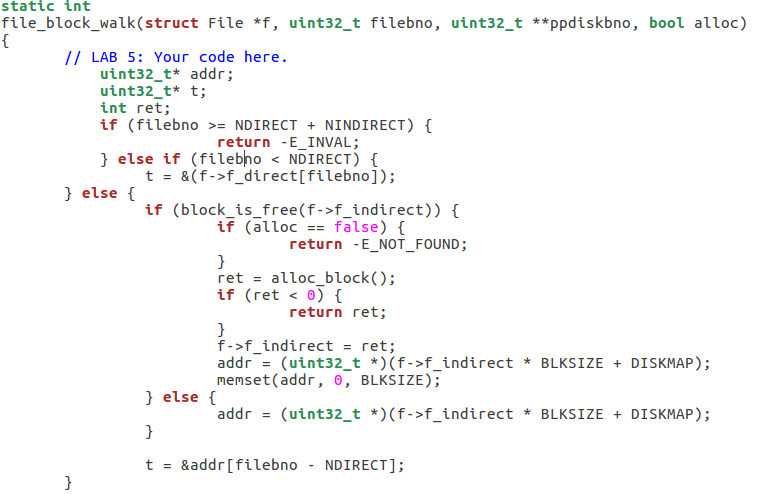
\includegraphics[width=6in]{figures/lab5/image76.png}

  file\_get\_block函数先调用file\_walk\_block函数找到文件中的目标块,然后将其转换为地址空间中的地址赋值给blk。

  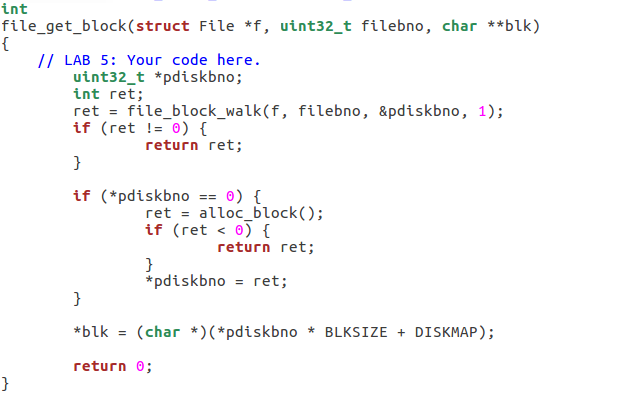
\includegraphics[width=6in]{figures/lab5/image77.png}

  \textbf{文件系统接口}

  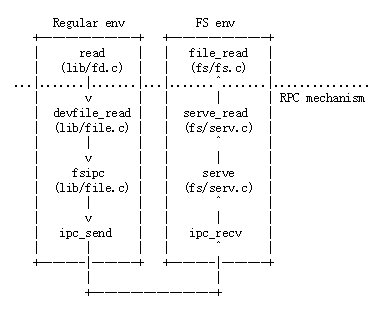
\includegraphics[width=6in]{figures/lab5/image78.png}

  实现了文件系统内的函数后,我们需要向外界提供更方便的统一接口。

  虚线下面的所有内容都是从常规环境到文件系统环境的读取请求的机制。read(提供的接口)在任何文件描述符上工作,并简单地调度到适当的设备读取功能,在这种情况下 devfile\_read(我们可以有更多的设备类型,如管道)。 devfile\_read 实现read专门针对磁盘上的文件。这个和lib / file.c中的其他devfile\_*函数 实现了FS操作的客户端,并且都以大致相同的方式工作,将请求结构中的参数捆绑在一起,调用 发送IPC请求,解包并返回结果。该fsipc 函数只是处理向服务器发送请求和接收答复的常见细节。

  文件系统服务器代码可以在fs / serv.c中找到。它在serve函数中循环通过IPC接收请求,将该请求分派给相应的处理函数,并通过IPC发回结果。在读取的例子中, serve将调度到serve\_read,将处理特定的IPC细节读取请求,如解开请求结构,最后调用 file\_read实际执行文件读取。

  JOS的IPC机制让一个环境发送一个单一的32位数字,并可选择共享一个页面。为了将请求从客户端发送到服务器,我们使用32位数字作为请求类型(文件系统服务器的RPC编号,就像syscalls的编号一样)并将参数存储union Fsipc在页面上的请求中 通过IPC共享。在客户端,我们总是共享页面fsipcbuf; 在服务器端,我们在fsreq (0x0ffff000)处映射传入的请求页面。

  服务器也通过IPC发回响应。我们使用32位数字作为函数的返回码。对于大多数RPC,这是他们所有的返回值。 FSREQ\_READ并FSREQ\_STAT返回数据,他们只是写入客户端发送请求的页面。在响应IPC中不需要发送此页面,因为客户端首先将其与文件系统服务器共享。此外,在答复中,FSREQ\_OPEN与客户分享一个新的“Fd页”。我们很快会返回到文件描述符页面。

  观察服务端主循环轮询时处理文件操作的过程:

  \begin{enumerate}
  \item 从IPC接受1个请求类型req以及数据页fsreq
  \item 然后根据req来执行相应的服务端处理函数
  \item 将相应服务端函数的执行结果(如果产生了数据也则有pg)通过IPC发送回调用进程
  \item 将映射好的物理页fsreq取消映射
  \end{enumerate}

  \Exercise{Serve\_read函数用于读文件请求。从ipc结构体中获取需要读取的目标信息,调用file\_read函数读取文件放置在ret\_buf中。}

  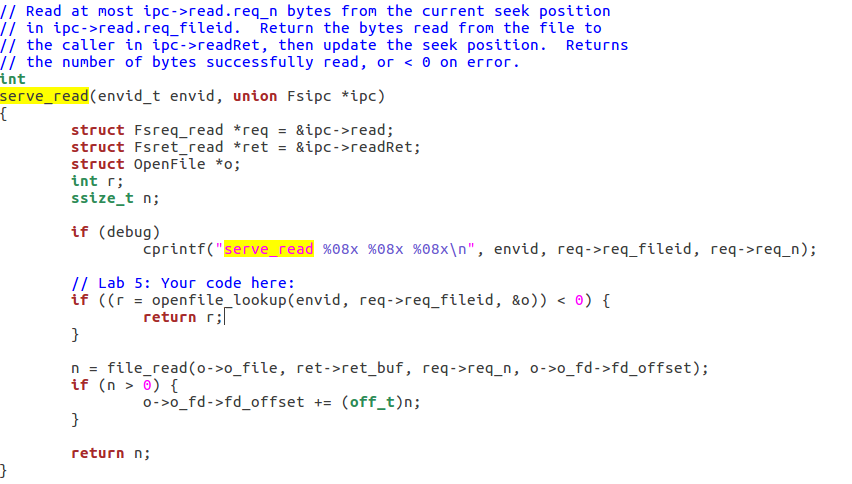
\includegraphics[width=6in]{figures/lab5/image80.png}

  \Exercise{serve\_write同样是获取请求信息,将req\_buf中的文件内容写入到磁盘块。}

  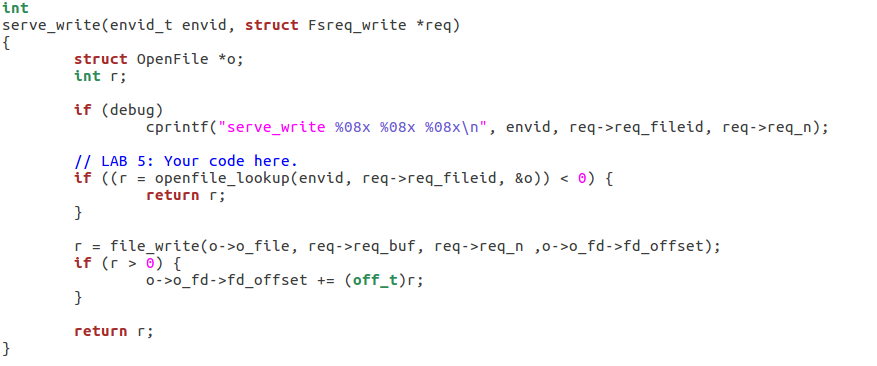
\includegraphics[width=6in]{figures/lab5/image83.png}

  Devfile\_write函数主要功能是将写文件需求通过fsipc打包成请求以便于发送给文件服务系统。

  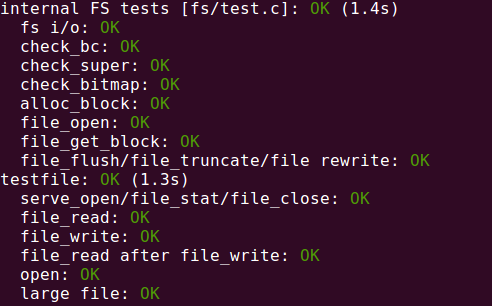
\includegraphics[width=6in]{figures/lab5/image84.png}

  \subsubsection{第二部分:Spawning过程}

  \textbf{环境继承}

  Spawn函数可以从父进程中调用,装载一个新的程序执行,类似于UNIX的fork后直接exec装载新的程序。
  Exercise7

  sys\_env\_set\_trapframe将父进程的环境(寄存器)复制为子进程的环境。

  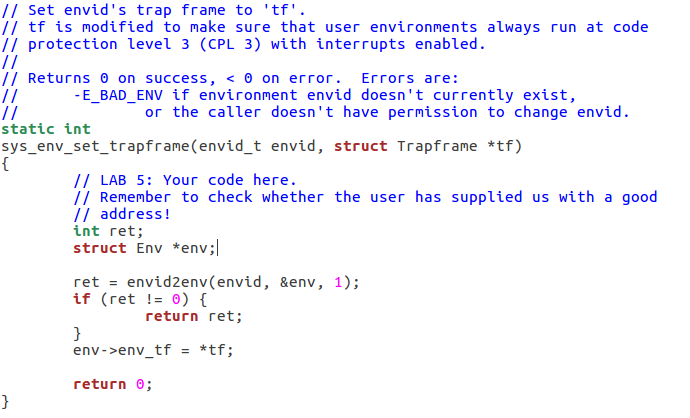
\includegraphics[width=6in]{figures/lab5/image86.png}

  加入系统调用

  
\includegraphics[width=6in]{figures/lab5/image87.png}

  使用make run-spawnhello可以看到父进程的信息和子进程的信息都输出了,输出中间的fs文件系统检查内容是由于多进程交替执行输出到控制台的结果。

  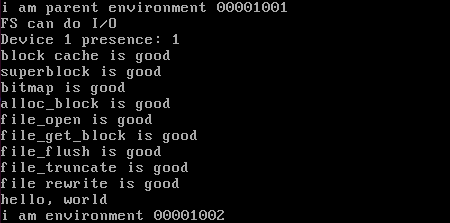
\includegraphics[width=6in]{figures/lab5/image88.png}

  \textbf{在fork和spawn之间共享库状态}

  UNIX文件描述符包括pipe,console I/O。 在JOS中,这些设备类型都有1个与与它关联的struct Dev,里面有实现read/write等文件操作的函数指针。在lib/fd.c中实现了传统UNIX的文件描述符接口。

    在lib/fd.c中也包括每个客户进程的文件描述符表布局,开始于FSTABLE。这块空间为每个描述符保留了1个页的地址空间。 在任何时候,只有当文件描述符在使用中才在文件描述符表中映射页。

    我们想要共享文件描述符状态在调用fork和spawn创建新进程。当下,fork函数使用COW会将状态复制1份而不是共享。在spawn中,状态则不会被拷贝而是完全舍弃。

    所以我们将改变fork来共享状态。在inc/lib.h中新定义了PTE\_SHARE位来标识页共享。当页表入口中设置了该位,则在fork和spawn时应该从父进程中拷贝PTE映射到子进程。

  \Exercise{在duppage中添加对PTE\_SHARE位进行判断,若有PTE\_SHARE位则直接复制映射。}

  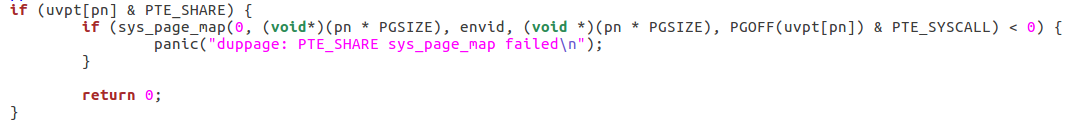
\includegraphics[width=6in]{figures/lab5/image90.png}

  在copy\_shared\_pages中扫描进程中所有页,发现PTE\_SHARE标记时,调用sys\_page\_map进行映射复制。

  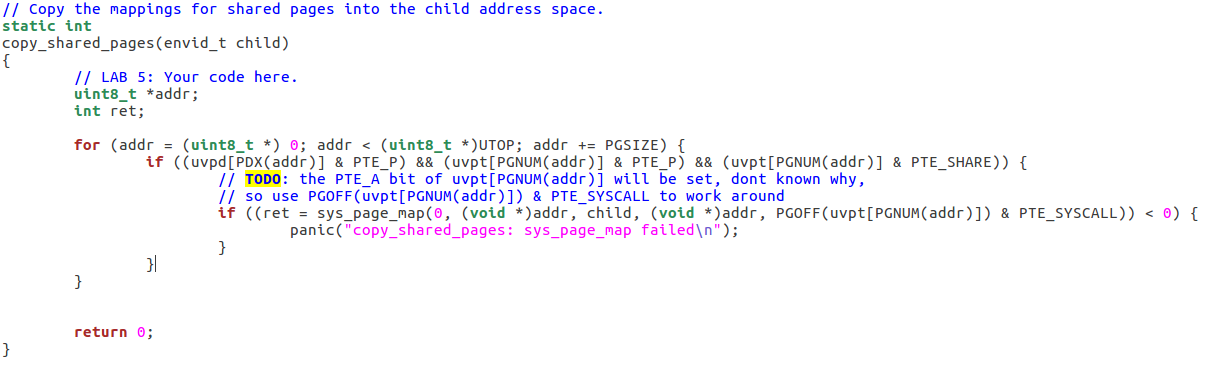
\includegraphics[width=6in]{figures/lab5/image91.png}

  运行make run-testpteshare,可以看到"fork handles PTE\_SHARE right" 和 "spawn handles PTE\_SHARE right"

  运行make run-testfdsharing,可以看到"read in child succeeded" 和 "read in parent succeeded"

  \subsubsection{第三部分:Shell}

  \textbf{键盘接口}

  为了使shell工作,我们需要一种方法来输入它。QEMU一直在显示我们写到CGA显示器和串行端口的输出,但到目前为止,我们只在内核监视器上进行输入。在QEMU中,输入在图形窗口中的输入显示为从键盘到JOS的输入,而输入到控制台的输入在串行端口上显示为字符。 kern / console.c已经包含了自实验1以来已被内核监视器使用的键盘和串口驱动程序,但是现在我们需要将这些驱动程序附加到系统的其他部分。

  \Exercise{在trap.c中添加对于IRQ\_OFFSET+IRQ\_KBD和IRQ\_OFFSET+IRQ\_SERIAL的判断,分别调用kbd\_intr和serial\_intr进行处理。}

  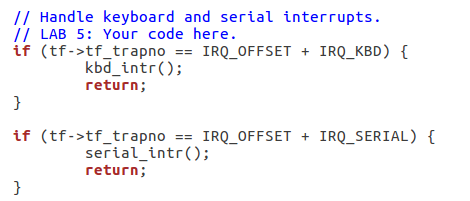
\includegraphics[width=6in]{figures/lab5/image96.png}

  运行make run-testkbd测试:

  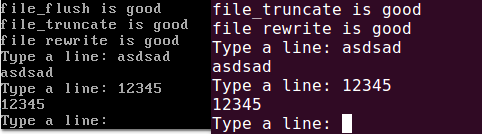
\includegraphics[width=6in]{figures/lab5/image97.png}

  \textbf{Shell命令}

  首先运行make run-icode测试

  echo hello world | cat 将hello world文本传送给cat程序,cat程序用来显示文本

  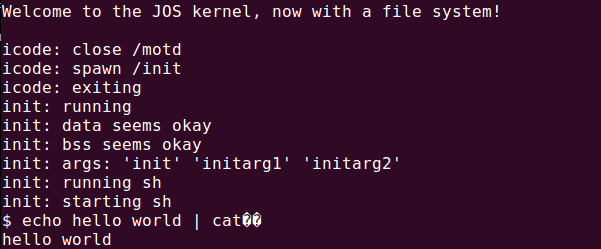
\includegraphics[width=6in]{figures/lab5/image98.png}

  cat lorem |cat 显示文本再传送给cat

  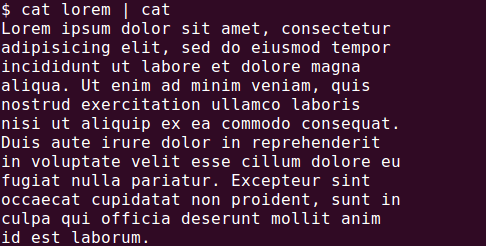
\includegraphics[width=6in]{figures/lab5/image99.png}

  cat lorem |num 给文本加上行号

  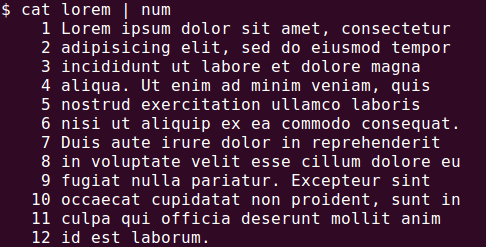
\includegraphics[width=6in]{figures/lab5/image100.png}

  cat lorem |num |num |num |num |num将加上行号的文本作为新文本再添加行号,多次迭代

  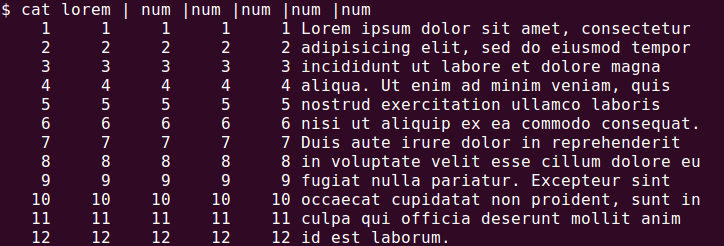
\includegraphics[width=6in]{figures/lab5/image101.png}

  lsfd

  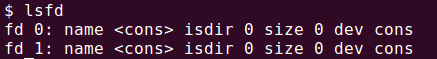
\includegraphics[width=6in]{figures/lab5/image102.png}

  \Exercise{要求我们实现shell的重定向特性,使用open()打开文件来获得命令输入。}

  运行make run-testshell来测试shell功能,成功重定向。

\end{ExerciseList}
